%
% komplex.tex -- Komplexe Differentialgleichungen
%
% (c) 2015 Prof Dr Andreas Mueller, Hochschule Rapperswil
%
\chapter{Komplexe Differentialgleichungen\label{chapter:komplexeanalysis}}
\lhead{}
\rhead{Komplexe Differentialgleichungen}
Die bisher betrachteten Differentialgleichungen waren immer f"ur
$x\in\mathbb R$ definiert.
Bei der L"osung mit Hilfe von Potenzreihen haben wir L"osungsfunktionen
gefunden, die man auch f"ur komplexe $x$-Werte auswerten kann.
Definiert man die Ableitung einer Funktionen einer komplexen Variablen
$z$ rein formal als
\[
\frac{d}{dz}z^n= nz^{n-1},
\]
dann kann man auch Potenzreihen in der Variablen $z$ formal differenzieren,
indem man jeden Term der Potenzreihe ableitet.
Und die mit der Potenzreihen-Methode gefunden L"osungen erf"ullen dann
auch die urspr"ungliche Differentialgleichung.
Dies ist aber eine rein formale "Uberlegung, da die Ableitung nach einer
komplexen Variablen noch gar nicht definiert ist.

%
% Komplex differenzierbare Funktion
%
\section{Komplex differenzierbare Funktionen}
Wir betrachten in diesem Kapitel komplexwertige Funktionen,
die ein einem Teilgebiet der komplexen Ebene definiert sind.
Ein {\em Gebiet} ist eine offene Teilmenge $\Omega\subset \mathbb C$.
{\em Offen} heisst, dass mit jedem Punkt $z_0\in\Omega$ eine Umgebung
\[
U=\{z\in\mathbb Z\,|\,|z-z_0|<\varepsilon\}
\]
ebenfalls in $\Omega$ enthalten ist, also $U\subset \Omega$ f"ur gen"ugen
kleines $\varepsilon$.
Sei also $f(z)$ eine in $\Omega\subset\mathbb C$ definierte
Funktion $f\colon\Omega\to\mathbb C$. 

Eine komplexwertige Funktion $f(z)$ kann betrachtet werden als zwei
reellwertige Funktionen von zwei Variablen $x$ und $y$:
\[
f(z)=\operatorname{Re}f(x+iy) + i \operatorname{Im}f(x+iy)
\]
Schreibt man
$\operatorname{Re}f(x+iy)=u(x,y)$
und
$\operatorname{In}f(x+iy)=v(x,y)$,
dann ist die komplexe Funktion vollst"andig durch reelle Funktionen
beschrieben.
Und nat"urlich wissen wir auch, was unter den Ableitungen der Funktionen 
$u(x,y)$ und $v(x,y)$ zu verstehen ist.
Der Funktion $f(z)$ entspricht eine Abbildung $\mathbb R^2\to\mathbb R^2$
\[
(x,y)\mapsto\begin{pmatrix}u(x,y)\\v(x,y)\end{pmatrix}.
\]
Die Ableitung einer solchen Funktion im Punkt $(x_0,y_0)$
ist eine lineare Abbildung von Vektoren, die in linearer N"aherung
den Funktionswert bei $f(z_0 + \Delta z)$ 
\[
\begin{pmatrix}
u(x+\Delta x, y +\Delta y)\\
v(x+\Delta x, y +\Delta y)
\end{pmatrix}
=
\begin{pmatrix}
\frac{\partial u}{\partial x}&\frac{\partial u}{\partial y}\\
\frac{\partial v}{\partial x}&\frac{\partial v}{\partial y}
\end{pmatrix}
\begin{pmatrix} \Delta x\\\Delta y \end{pmatrix}
+o(\Delta x, \Delta y).
\]
In dieser Sicht einer komplexen Funktion gibt es keine einzelne Zahl, die
die Funktion einer Ableitung "ubernehmen k"onnte, die Ableitung
ist eine $2\times 2$-Matrix.

%
% Definition der komplexen Ableitungen
%
\subsection{Komplexe Ableitung}
Die Ableitung einer Funktion einer reellen Variablen wird mit Hilfe des
Grenzwertes
\[
f'(x_0)=\lim_{x\to x_0}\frac{f(x)-f(x_0)}{x-x_0}
\]
definiert, oder als diejenige Zahl $f'(x_0)\in\mathbb R$ mit der Eigenschaft,
dass
\begin{equation}
f(x)=f(x_0)+f'(x_0)(x-x_0) + o(x-x_0)
\label{komplex:abldef}
\end{equation}
gilt.
Der Term $x-x_0$ und die Gleichung (\ref{komplex:abldef}) sind aber auch
f"ur komplexe Argument sinnvoll, wir definieren daher

\begin{definition}
Die komplexe Funktion $f(z)$ heisst im Punkt komplex differenzierbar
und hat die komplexe Ableitung $f'(z_0)\in\mathbb C$,
wenn 
\begin{equation}
f(z)=f(z_0) + f'(z_0)(z-z_0) +o(z-z_0)
\label{komplex:defkomplabl}
\end{equation}
gilt.
\end{definition}

\begin{beispiel}
Die Funktion $z\mapsto f(z)=z^n$ ist "uberall komplex differenzierbar
und hat die Ableitung $nz^{n-1}$.
Um dies nachzupr"ufen, m"ussen wir die Bedingung~(\ref{komplex:defkomplabl})
verifizieren.
Aus einer wohlbekannten Faktorisierung von $z^n - z_0^n$ k"onnen wir den
Differenzenquotienten finden:
\[
\frac{f(z)-f(z_0)}{z-z_0}
=
\frac{z^n-z_0^n}{z-z_0}
=
\frac{(z-z_0)(z^{n-1}+z^{n-2}z_0+z^{n-3}z_0^2+\dots+z^{n-1})}{z-z_0}
=
z^{n-1}+z^{n-2}z_0+z^{n-3}z_0^2+\dots+z^{n-1}
\]
Lassen wir jetzt $z$ gegen $z_0$ gehen, wird die rechte Seite
zu $nz_0^{n-1}$.
\end{beispiel}

\begin{beispiel}
Die Funktion $z\mapsto f(z)=\bar z=x-iy$ ist nicht differenzierbar.
Wenn $f(z)=\bar z$ differenzierbar w"are, dann m"usste es eine Zahl
$a\in\mathbb C$ geben, so dass 
\[
\bar z-\bar z_0=a(z-z_0)+o(z-z_0)
\]
gilt.
w"ahlen wir $z=z_0+x$ bzw.~$z=z_0+iy$, dann erhalten wir
\[
\begin{aligned}
z-z_0&=x:&
\bar z-\bar z_0&=x
&&\Rightarrow&
\bar z-\bar z_0&=1\cdot x
&&\Rightarrow&
a&=1
\\
z-z_0&=iy:&
\bar z-\bar z_0&=-iy
&&\Rightarrow&
\bar z-\bar z_0&=-1\cdot iy
&&\Rightarrow&
a&=-1
\end{aligned}
\]
Es ist also nicht m"oglich, eine einzige Zahl $a$ zu finden, die als
die Ableitung der Funktion $z\mapsto \bar z$ betrachtet werden k"onnte.
\end{beispiel}

Das letzte Beispiel zeigt, dass
selbst Funktionen, deren Real- und Imagin"arteil beliebig oft stetig
differenzierbare Funktionen sind, nicht komplex differenzierbar
sein m"ussen.
Komplexe Differenzierbarkeit ist eine wesentlich st"arkere Bedingung
an eine Funktion, komplex differenzierbare Funktionen bilden eine
echte Teilmenge aller Funktionen, deren Real- und Imagin"arteil
differenzierbar ist.

%
% Cauchy-Riemann-Differentialgleichungen
%
\subsection{Die Cauchy-Riemann-Differentialgleichungen}
Komplexe Funktionen k"onnen nur differenzierbar sein, wenn sich die vier
partiellen Ableitungen zu einer einzigen komplexen Zahl zusammenfassen
lassen.
Um diese Beziehung zu finden, gehen wir von einer komplexen Funktion
\[
f(x+iy) = u(x,y) + iv(x,y)
\]
aus, und berechnen die Ableitung auf zwei verschiedene Arten, indem
wir sowohl nach $x$ als auch nach $iy$ ableiten:
\begin{align*}
f'(z)&
=
\lim_{x\to 0}\frac{f(z+x)-f(z)}{x}
=
\frac{\partial u}{\partial x}+i\frac{\partial v}{\partial x}
\\
f'(z)&
=
\lim_{y\to 0}\frac{f(z+iy)-f(z)}{iy}
=
\frac1{i}
\frac{\partial u}{\partial y}+\frac{\partial v}{\partial y}
=
\frac{\partial v}{\partial y}
-i
\frac{\partial u}{\partial y}.
\end{align*}
Dies ist nur m"oglich, wenn Real- und Imagin"arteile "ubereinstimmen.
Es folgt also

\begin{satz}
\label{komplex:satz:cauchy-riemann}
Real- und Imagin"arteil $u(x,y)$ und $v(x,y)$ einer
komplex differenzierbaren Funktion $f(z)$ mit $f(x+iy)=u(x,y)+iv(x,y)$
erf"ullen die Cauchy-Riemannschen Differentialgleichungen
\index{Cauchy-Riemann-Differentialgleichungen}
\begin{equation}
\begin{aligned}
\frac{\partial u}{\partial x}
&=
\frac{\partial v}{\partial y},
&
\frac{\partial u}{\partial y}
&=
-
\frac{\partial v}{\partial x}
\end{aligned}
\label{komplex:dgl:cauchy-riemann}
\end{equation}
\end{satz}

Leitet man die Cauchy-Riemann-Differentialgleichungen nochmals nach
$x$ und $y$ ab, erh"alt man
\begin{equation*}
\begin{aligned}
\frac{\partial^2 u}{\partial x^2}
&=
\frac{\partial^2 v}{\partial x\,\partial y},
&
\frac{\partial^2 u}{\partial x\,\partial y}
&=
-\frac{\partial^2 v}{\partial x^2},
&
\frac{\partial^2 u}{\partial y\,\partial x}
&=
\frac{\partial^2 v}{\partial y^2},
&
\frac{\partial^2 u}{\partial y^2}
&=
-\frac{\partial^2 v}{\partial y\,\partial x}.
\end{aligned}
\end{equation*}
Die erste und die letzte sowie die mittleren zwei k"onnen zu jeweils
einer Differentialgleichung f"ur die Funktionen $u$ und $v$ zusammengefasst
werden, n"amlich
\begin{equation*}
\frac{\partial^2 u}{\partial x^2}
+
\frac{\partial^2 u}{\partial y^2}
=
0
\qquad\text{und}\qquad
\frac{\partial^2 v}{\partial x^2}
+
\frac{\partial^2 v}{\partial y^2}
=
0
\end{equation*}

\begin{definition}
Der Operator 
\[
\Delta =
\frac{\partial^2}{\partial x^2}
+
\frac{\partial^2}{\partial y^2}
\]
heisst der {\em Laplace-Operator} in zwei Dimensionen
\index{Laplace-Operator}.
\end{definition}

\begin{definition}
Eine Funktion $h(x,y)$ von zwei Variablen heisst {\em harmonisch}, wenn sie
die Gleichung
\[
\Delta h=0
\]
erf"ullt.
\index{harmonische Funktion}
\end{definition}

\begin{satz}
Real- und Imagin"arteil einer komplexen Funktion sind harmonische Funktionen.
\end{satz}

Die Cauchy-Riemann-Differentialgleichungen schr"anken also einerseits stark
ein, welche Funktionen "uberhaupt als Real- und Imagin"arteil einer
komplex differenzierbaren Funktion in Frage kommen.
Andererseits koppeln sie auch Real- und Imagin"arteil stark zusammen.

\begin{beispiel}
Von einer komplex differenzierbaren Funktion $f(z)$ sei nur der Realteil
$u(x,y)=x^3 -3xy^2$ bekannt.
Zun"achst kontrollieren wir, ob dies "uberhaupt ein Realteil sein kann,
indem wir nachrechnen, ob $u(x,y)$ harmonisch ist.
\begin{equation*}
\begin{aligned}
\frac{\partial u}{\partial x}
&=
3x^2-3y^2
&&\Rightarrow&
\frac{\partial^2 u}{\partial x^2}
&=
6x
\\
\frac{\partial u}{\partial y}
&=
-6xy
&&\Rightarrow&
\frac{\partial^2 u}{\partial y^2}
&=
-6x
\\
&&&&\Delta u&=\frac{\partial^2u}{\partial x^2}+\frac{\partial^2u}{\partial y^2}=6x-6x=0,
\end{aligned}
\end{equation*}
$u$ ist also harmonisch.
Um die Funktion $f$ zu finden, brauchen wir jetzt noch den Imagin"arteil.
Wir finden ihn mit Hilfe der Cauchy-Riemann-Differentialgleichungen.
Es gilt
\begin{equation}
\begin{aligned}
\frac{\partial v}{\partial x}
&=
-\frac{\partial u}{\partial y}=6xy,
&
\frac{\partial v}{\partial y}
&=
\frac{\partial u}{\partial x}=3x^2-3y^2
\end{aligned}
\label{komplex:crbeispiel}
\end{equation}
Aus der ersten Gleichung erh"alt man durch Integrieren nach $x$ 
\[
v(x,y)=-3x^2y + C(y),
\]
die Integrations-``Konstante'' ist eine Funktion, die aber nur von $y$
abh"angen darf.
Die zweite Cauchy-Riemann-Gleichung verwendet die Ableitung von $v$ nach $y$,
sie ist
\[
\frac{\partial v}{\partial y}=3x^2+C'(y).
\]
Aus der zweiten Gleichung von (\ref{komplex:crbeispiel}) liest man
ab, dass
\[
C'(y)=-3y^2
\qquad\Rightarrow\qquad
C(y)=-y^3+k
\]
sein muss.
Damit ist $v$ bis auf eine Konstante bestimmt.
Die zugeh"orige Funktion $f(z)$ ist daher
\[
f(z)=f(x+iy)=x^3-3xy^2+i(3x^2y-y^3)+ik
=x^3 + 3x^2iy + 3x(iy)^2+(iy)^3+ik=z^3+ik.
\]
Wir haben die Funktion $f(z)$ bis auf eine Konstanten $ik$ 
aus ihrem Realteil rekonstruiert.
\end{beispiel}

Die Cauchy-Riemann-Differentialgleichungen besagen auch, dass man nur
die Ableitungen nach $x$ zu berechnen braucht, um die Ableitung $f'(x)$
zu bestimmen.
Die Rechenregeln f"ur die Ableitung lassen sich daher direkt auf
komplexe Funktionen "ubertragen.
\begin{align*}
\frac{d}{dz}z^n
&=
nz^{n-1}
\\
\frac{d}{dz}e^z
&=
e^z
\\
\frac{d}{dz}f(g(z))
&=
f'(g(z)) g'(z)
\\
\frac{d}{dz}\bigl(f(z)g(z)\bigr)
&=
f'(z)g(z)+f(z)g'(z)
\end{align*}

%
% Analytische Funktionen
%
\subsection{Analytische Funktionen}
Als wichtiges Beispiel komplex differenzierbarer Funktionen betrachten
wir die analytischen Funktionen.
\begin{definition}
Eine Funktion $f\colon\mathbb C\to\mathbb C$ heisst analytisch im Punkt
$z_0$, wenn sie in eine konvergente Potenzreihe
\begin{equation}
f(z)=\sum_{k=0}^\infty a_k(z-z_0)^k
\label{komplex:freihe}
\end{equation}
entwickelt werden kann.
\end{definition}

Da die Ableitungsregeln f"ur komplex differenzierbare Funktionen nicht
anders sind als die Ableitungsregeln f"ur relle Funktionen, muss gelten
\begin{equation}
f'(z)=\sum_{k=1}^\infty ka_k(z-z_0)^{k-1},
\label{komplex:fpreihe}
\end{equation}
und es stellt sich nur die Frage, ob diese Potenzreihe ebenfalls konvergent
ist.
Man kann dies mit der Formel f"ur den Konvergenzradius pr"ufen.
F"ur die Potenzreihe (\ref{komplex:freihe}) f"ur $f(z)$ liefert sie den
Konvergenzradius
\[
\frac{1}{\varrho} = \limsup_{k\to\infty} \root{k}\of{|a_k|}.
\]
Dieselbe Formel f"ur die Reihe~(\ref{komplex:fpreihe}) liefert
f"ur den Konvergenzradius der Ableitung $f'(z)$
\[
\limsup_{k\to\infty} \root{k}\of{k|a_k|}
=
\underbrace{\lim_{k\to\infty} \root{k}\of{k}}_{\textstyle=1}
\cdot
\underbrace{ \limsup_{k\to\infty} \root{k}\of{|a_k|}}_{\textstyle=1/\varrho}
=
\frac1{\varrho}.
\]
Die Reihe f"ur die Ableitung $f'(z)$ hat also den gleichen Konvergenzradius
wie die Reihe f"ur die Funktion $f(z)$, dies gilt nat"urlich auch f"ur
die h"oheren Ableitungen.

Eine analytische Funktion ist somit beliebig oft komplex differenzierbar.
Aus den Ableitungen kann wie bei reellen Funktionen die Taylor-Reihe
gebildet werden, sie muss mit der Potenzreihe (\ref{komplex:freihe})
"ubereinstimmen.
Analytische Funktionen haben also eine konvergente Tayler-Reihe,
\[
f(z) = \sum_{k=0}^\infty \frac{f^{(k)}(z_0}{k!}(z-z_0)^k.
\]

%
% Wegintegrale und die Cauchy-Formel
%
\subsection{Wegintegrale\label{subsection:wegintegrale}}
Das Finden einer Stammfunktion, die Integration, ist die Grundtechnik,
mit der man den "Ubergang von lokaler Information in Form von Ableitungen,
zu globaler Information "uber reelle Funktionen vollzieht.
Sie liefert aus der Steigung zwischen zwei Punkten $x_0$ und $x$ den
Funktionswert mittels
\[
f(x)=f(x_0)+\int_{x_0}^xf'(\xi)\,d\xi.
\]
Bei einer reellen Funktion gibt es nur eine Richtung, entlang der man
integrieren k"onnte.

Auch in der komplexen Ebene erwarten wir eine Formel
\[
f(z) = f(z_0) + \int_{z_0}^z f'(\zeta)\,d\zeta.
\]
In der komplexen Ebene gibt es aber beliebig viele Wege, mit denen die
Punkte $z_0$ und $z$ verbunden werden k"onnen. 
Der Wert von $f(z)$ muss also durch Integration entlang eines speziell
gew"ahlten Weges $\gamma$
\[
f(z) = f(z_0) + \int_{\gamma} f'(\zeta)\,d\zeta
\]
bestimmt werden.
Es muss also zun"achst gekl"art werden, wie ein solches Wegintegral
"uberhaupt zu verstehen und zu berechnen ist.
Dann gilt es zu untersuchen, inwieweit diese Konstruktion unabh"angig
von der Wahl des Weges ist.
F"ur komplex differenzierbare Funktionen wird sich eine sehr erfolgreiche
Theorie ergeben.

%
% Wegintegrale
%
\subsubsection{Definition des Wegintegrals}
Ein Weg in der komplexen Ebene ist eine Abbildung 
\[
\gamma\colon [a,b]\to\mathbb C: t\mapsto \gamma(t).
\]
Wir verlangen f"ur unsere Zwecke zus"atzlich, dass $\gamma$ differenzierbar
ist.
Dann k"onnen wir f"ur jede beliebige Funktion das Wegintegral definieren.

\begin{definition}
Sei $\gamma\colon[a,b]\to\mathbb C$ ein Weg in $\mathbb C$ und $f(z)$
eine stetige komplexe Funktion, dann heisst
\[
\int_{\gamma} f(z)\,dz = \int_a^bf(\gamma(t)) \gamma'(t)\,dt
\]
das {\em Wegintegral} von $f(z)$ entlang der Kurve $\gamma$.
\index{Wegintegral}
\end{definition}

\begin{beispiel}
Wir berechnen als Beispiel das Wegintegral der Funktion $f(z)=1/z$ entlang
eines Halbkreises von $1$ zu $-1$. 
Es gibt zwei verschiedene solche Halbkreise:
\begin{equation*}
\begin{aligned}
\gamma_+(t)&=e^{it},&t&\in[0,\pi]
\\
\gamma_-(t)&=e^{-it},&t&\in[0,\pi]
\end{aligned}
\end{equation*}
Wir finden f"ur die Wegintegrale
\begin{align*}
\int_{\gamma_+}\frac1z\,dz
&=
\int_0^\pi \frac1{e^{it}}ie^{it}\,dt=i\int_0^\pi\,dt=i\pi
\\
\int_{\gamma_-}\frac1z\,dz
&=
-\int_0^\pi \frac1{e^{-it}}ie^{-it}\,dt=-i\int_0^\pi\,dt=-i\pi
\end{align*}
Das Wegintegral zwischen $1$ und $-1$ h"angt also mindestens f"ur diese
spezielle Funktion $f(z)=1/z$ von der Wahl des Weges ab.
\end{beispiel}

Wie Wahl der Parametrisierung der Kurve hat keinen Einfluss auf den 
Wert des Wegintegrals.

\begin{satz}
Seien $\gamma_1(t), t\in[a,b],$ und $\gamma_2(s),s\in[c,d]$
verschiedene Parametrisierungen
der gleichen Kurve, es gebe also eine Funktion $t(s)$ derart, dass
$\gamma_1(t(s))=\gamma_2(s)$.
Dann ist
\[
\int_{\gamma_1}f(z)\,dz
=
\int_{\gamma_2}f(z)\,dz.
\]
\end{satz}

\begin{proof}[Beweis]
Wir verwenden die Definition des Wegintegrals
\begin{align*}
\int_{\gamma_1} f(z)\,dz
&=
\int_a^b f(\gamma_1(t))\,\gamma_1'(t)\,dt
=
\int_c^d f(\gamma_1(t(s))\,\underbrace{\gamma_1'(t(s)) t'(s)}_{\displaystyle
=\frac{d}{ds}\gamma_1(t(s))}\,ds
\\
&=
\int_c^d f(\gamma_2(s)\,\gamma_2'(s)\,ds
=
\int_{\gamma_2}f(z)\,dz
\end{align*}
Beim zweiten Gleichheitszeichen haben wir die Formel f"ur die
Variablentransformation $t=t(s)$ in einem Integral verwendet.
\end{proof}

Wir erwarten, dass das Wegintegral "ahnlich wie das Integral reeller
Funktionen eine Art ``Umkehroperation'' zur Ableitung ist.
Wir untersuchen daher den Fall, dass $f(z)$ eine komplexe Stammfunktion $F(z)$
hat, also $f(z)=F'(z)$.
Wir berechnen das Wegintegral entlang des Weges $\gamma$:
\begin{align*}
\int_{\gamma}f(z)\,dz
&=
\int_a^bf(\gamma(t))\,\gamma'(t)\,dt
=
\int_a^bF'(\gamma(t))\,\gamma'(t)\,dt
=
\int_a^b\frac{d}{dt}F(\gamma(t))\,dt
=
F(\gamma(a))-F(\gamma(b))
\end{align*}
Dies ist genau die Formel, die man als den Hauptsatz der Infinitesimalrechnung
kennt.
Trotzdem ist die Situation hier etwas anders.
In der reellen Infinitesimalrechnung war die Existenz einer Stammfunktion
durch das Integral gesichert, man konnte mit
\[
F(x)=\int_a^xf(\xi)\,d\xi
\]
immer eine Stammfunktion angeben.
Im komplexen Fall k"onnen wir nat"urlich auch versuchen, eine Stammfunktion
mit Hilfe von 
\[
F(z)=\int_{\gamma_z} f(\zeta)\,d\zeta
\]
zu definieren.
Dabei muss allerdings $\gamma_z$ ein Weg sein, der im Punkt $z$ endet,
und wir wissen noch nicht einmal, ob die Wahl des Weges eine Rolle
spielt.
Bevor wir also sicher sein k"onnen, dass eine Stammfunktion existiert,
m"ussen wir zeigen, dass das Wegintegral einer komplex differenzierbaren
Funktion zwischen zwei Punkten nicht von der Wahl des Weges abh"angt,
der die beiden Punkte verbindet.
Dazu ist notwendig, geschlossene Wege genauer zu betrachten.

%
% Wegintegrale führen auf analytische Funktionen
%
\subsubsection{Wegintegrale f"uhren auf analytische Funktionen}
\begin{figure}
\centering
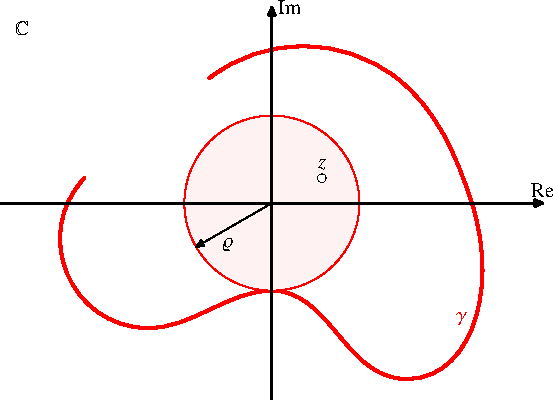
\includegraphics{chapters/images/komplex-4.pdf}
\caption{Pfad und Konvergenzradius f"ur den Nachweis, dass Wegintegrale
auf analytische Funktionen f"uhren (Satz~\ref{komplex:integralanalytisch})
\label{komplex:integralanalytischpfad}}
\end{figure}
Mit Wegintegralen kann man aus stetigen Funktionen neue Funktionen
konstruieren.
Die folgende Konstruktion liefert "uberraschenderweise immer
analytische Funktionen.
\begin{satz}
\label{komplex:integralanalytisch}
Sei $\gamma\colon [a,b]\to\mathbb C$ ein Weg in $\mathbb C$, der nicht
durch den Nullpunkt verl"auft, und $g$ eine stetige Funktion
auf $\gamma([a,b])$ (Abbildung~\ref{komplex:integralanalytischpfad}).
Dann ist die Funktion
\[
f(z) = \frac1{2\pi i}\int_\gamma \frac{g(x)}{x-z}\,dx
\]
in einer Umgebung des Nullpunktes analytisch:
\[
f(z) = \sum_{k=0}^\infty c_k z^k,\qquad
\text{mit\quad}
c_k=\frac1{2\pi i}\int_\gamma \frac{g(x)}{x^{k+1}}\,dx.
\]
Der Konvergenzradius $\varrho$ dieser Reihe ist der minimale Abstand der
Kurve $\gamma$ vom Nullpunkt.
\end{satz}

\begin{proof}[Beweis]
Zun"achst schreiben wir
\begin{equation}
\frac{1}{x-z}
=
\frac1x\cdot \frac{1}{1-\displaystyle\frac{z}{x}}
=
\frac1x\cdot \sum_{k=0}^\infty \biggl(\frac{z}{x}\biggr)^k
=
\sum_{k=0}^\infty \frac{z^k}{x^{k+1}}.
\label{komplex:georeihe}
\end{equation}
Damit k"onnen wir jetzt die Funktion $f(z)$ berechnen:
\begin{align*}
f(z)
&=
\frac1{2\pi i} \int_{\gamma} \frac{g(x)}{x-z}\,dx
=
\frac1{2\pi i} \int_{\gamma} \sum_{k=0}^\infty \frac{z^k}{x^{k+1}}g(x)\,dx
=
\sum_{k=0}^\infty
\underbrace{\biggl(\frac1{2\pi i} \int_{\gamma} \frac{g(x)}{x^{k+1}}\,dx\biggr)}_{\textstyle =c_k}
z^k
=
\sum_{k=0}^\infty c_kz^k.
\end{align*}
Wir m"ussen uns noch die Konvergenz dieser Reihen "uberlegen.
Wenn $z<\varrho$ ist, dann ist 
\[
\biggl|\frac{z}{x}\biggr| 
=
\frac{|z|}{|x|}
<1,
\]
so dass die geometrische Reihe (\ref{komplex:georeihe}) konvergent ist,
daraus lesen wir ab, dass der Konvergenzradius mindestens $\varrho$
ist.
Gr"osser kann er allerdings auch nicht sein, da f"ur $|z|\ge \varrho$
das Integral nicht mehr definiert sein muss.
Nimmt man n"amlich einen Punkt von $g([a,b])$ f"ur $z$ wird der Integrand
unendlich gross.
\end{proof}

Der Satz~\ref{komplex:integralanalytisch} ist nur f"ur Potenzreihen
im Punkt $0$ formuliert, was im Wesentlichen durch die
Umformung~(\ref{komplex:georeihe}) bedingt war.
Man kann dies aber auch als Potenzreihe
\[
\frac1{x-z}
=
\frac1{x-z_0-(z-z_0)}
=
\frac1{x-z_0}\cdot\frac{1-\frac{z-z_0}{x-z_0}}
=
\frac1{x-z_0}\sum_{k=0}^\infty\biggl(Ò\frac{z-z_0}{x-z_0}\biggr)^k
=
\sum_{k=0}^\infty\frac1{(x-z_0)^{k+1}}(z-z_0)^k
\]
im Punkt $z_0$ ausdr"ucken.
Man bekommt dann die Potenzreihe
\[
f(z) = \sum_{k=1}^\infty c_k(z-z_0)^k,\qquad
\text{mit}\quad
c_k=\frac1{2\pi i}\oint_\gamma\frac{g(x)}{(x-z_0)^{k+1}}\,dx
\]
f"ur das Wegintegral.

\subsubsection{Laurent-Reihen}
\begin{figure}
\centering
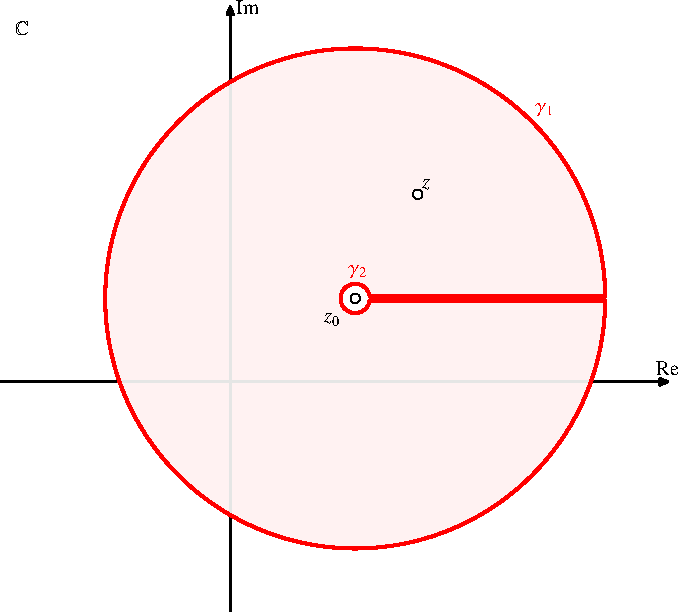
\includegraphics{chapters/images/komplex-3.pdf}
\caption{Pfad zur Herleitung der Laurent-Reihe einer Funktion $f(z)$
mit einer Singularit"at $z_0$.
\label{komplex:laurentpfad}}
\end{figure}%
In Satz~\ref{komplex:integralanalytisch} konnten wir eine Potenzreihe f"ur
solche $z$ konstruieren, deren Betrag kleiner ist als der kleinste Abstand
der Kurve $\gamma$ vom Ursprung.
Dies war notwendig, weil in~(\ref{komplex:georeihe}) die geometrische Reihe
nur konvergiert, wenn der Quotient $<1$ ist.
Wenn die Funktion $f(z)$ jedoch eine Singularit"at im Punkt $z_0$ hat, dann
kann es nicht m"oglich sein, die Funktion mit einer Potenzreihe zu
beschreiben.

Wir verwenden daher den speziellen Pfad in Abbildung~\ref{komplex:laurentpfad}.
Er f"uhrt in einem grossen Kreis $\gamma_1$ um den Punkt $z_0$ herum,
dann folgt ein zur $x$-Achse paralleler Abschnitt, der bis zum kleinen
Kreis $\gamma_2$ f"uhrt.
Nach Durchlaufen des kleinen Kreises $\gamma_2$ im Uhrzeigersinn folgt wieder
ein zur $x$-Achse paralleles St"uck zur"uck zum grossen Kreis.
Da die geraden St"ucke zweimal in entgegegengesetzer Richtung durchlaufen
werden, heben sie sich weg.
Ein Wegintegral entlang $\gamma$ zerf"allt daher in eine Differenz
\[
\oint_\gamma\dots\,dz
=
\oint_{\gamma_1}\dots\,dz
-
\oint_{\gamma_2}\dots\,dz
\]
von Wegintegralen entlang $\gamma_1$ und $\gamma_2$.

Der "aussere Pfad $\gamma_1$ gibt wie in Satz~\ref{komplex:integralanalytisch}
Anlass zu einer Potenzreihe in $(z-z_0)$.
Der innere Pfad $\gamma_2$ kann aber nicht so behandelt werden, da $z$ immer
weiter von $z_0$ entfernt als die Punkte auf $\gamma_2$.
Allerdings ist $|x/z| < 1$ f"ur Punkte auf $\gamma_2$, wir m"ussen daher
die geometrische Reihe auf $x/z$ anwenden:
\begin{align*}
\frac{1}{x-z}
&=
\frac{1}{x-z_0-(z-z_0)}
=
\frac{1}{z-z_0}
\cdot
\frac{1}{\displaystyle\frac{x-z_0}{z-z_0}-1}
=
-\sum_{k=0}^\infty \frac{(x-z_0)^k}{(z-z_0)^{k+1}}.
\end{align*}
Das Integral entlang der Kurve $\gamma_2$ kann also als Reihe in $1/(z-z_0)$
entwickelt werden:
\begin{align*}
f_2(z)
&=
\frac{1}{2\pi i}\int_{\gamma_2} \frac{g(x)}{x-z}\,dx
=
\frac{1}{2\pi i}\int_{\gamma_2}\sum_{k=0}^\infty
\frac{(x-z_0)^k}{(z-z_0)^{k+1}}\,dx
\\
&=
\sum_{k=0}^\infty
\biggl(
\underbrace{\frac1{2\pi i}\int_{\gamma_2} (x-z_0)^kg(x)\,dx
}_{\textstyle =d_{k+1}}
\biggr)
\frac1{(z-z_0)^{k+1}}
=\sum_{k=1}^\infty \frac{d_k}{(z-z_0)^k}.
\end{align*}
Zusammen mit der vom Integral entlang $\gamma_1$ herr"uhrenden Reihe finden
wir den Satz
\begin{satz}
\label{komplex:laurentreihe}
Ist $g(z)$ eine entlang der Kurve $\gamma$ wie in
Abbildung~\ref{komplex:laurentpfad} definierte stetige Funktion, dann gilt
\[
f(z)=\frac1{2\pi i}\oint_{\gamma} \frac{f(x)}{x-z}\,dx
=
\sum_{k=0}^{\infty} c_k(z-z_0)^k-\sum_{k=1}^\infty \frac{d_k}{(z-z_0)^k},
\]
wobei die Koeffizienten $c_k$ und $d_k$ gegeben sind durch
\[
\begin{aligned}
c_k&=\frac1{2\pi i}\oint_{\gamma_1} \frac{g(x)}{x-z_0}\,dx
&&
\text{und}
&
d_k&=\frac1{2\pi i}\oint_{\gamma_2} g(x)x^{k-1}\,dx.
\end{aligned}
\]
\end{satz}

\begin{definition}
Eine Reihe der Form
\[
\sum_{k=-\infty}^\infty a_k(z-z_0)^k
\]
heisst {\em Laurent-Reihe }
im Punkt $z_0$.
\end{definition}


%
% Geschlossene Wege
%
\subsubsection{Geschlossene Wege}
\begin{definition}
Ein Weg $\gamma\colon[a,b]\to\mathbb C$ heisst {\em geschlossen}, wenn
$\gamma(a)=\gamma(b)$.
\index{geschlossener Weg}
Das Integral entlang eines geschlossenen Weges h"angt nicht von der
Parametrisierung ab und wird zur Verdeutlichung mit
\[
\int_{\gamma}f(z)\,dz
=
\oint_{\gamma}f(z)\,dz
\]
bezeichnet.
\end{definition}

\begin{beispiel}
Wir berechnen das Integral von $f(z)=z^n$ entlang des Einheitskreises,
den wir mit $\gamma(t)=e^{it},t\in[0,2\pi]$ parametrisieren.
Die Definition liefert:
\begin{align*}
\oint_{\gamma}f(z)\,dz
&=
\int_0^{2\pi}e^{int}ie^{it}\,dt
=
i\int_0^{2\pi}e^{i(n+1)t}\,dt
\end{align*}
F"ur $n=-1$ ist dies das Integral einer konstanten Funktion, also
\[
\oint_{\gamma}\frac1z\,dz=2\pi i.
\]
F"ur $n\ne -1$ kann man eine Stammfunktion von $e^{i(n+1)t}$
verwenden:
\[
\oint_{\gamma}f(z)\,dz
=
i\left[\frac1{i(n+1)}e^{i(n+1)t}\right]_0^{2\pi}
=0,
\]
weil $e^{i(n+1)t}$ periodisch ist mit Periode $2\pi$.
\end{beispiel}
Das Beispiel zeigt, dass ein Wegintegral der Potenzfunktionen,
aller Polynome und schliesslich aller konvergenten Potenzreihen
"uber einen geschlossenen Weg verschwinden.
Es zeigt aber auch, dass das Wegintegral "uber einen geschlossenen
Weg nicht zu verschwinden braucht, wie das Beispiel $f(z)=1/z$ 
zeigt.
Letztere Funktion unterscheidet sich von den Potenzfunktionen allerdings
dadurch, dass sie im Nullpunkt nicht definiert ist.

\begin{satz}
Sei $f(z)$ eine in einem zusammenh"angenden Gebiet $\Omega\subset\mathbb C$
definierte komplexe Funktion, f"ur die das Wegintegral "uber jeden
geschlossenen Weg verschwindet.
Dann hat $f(z)$ eine komplexe Stammfunktion $F(z)$.
\end{satz}

\begin{proof}[Beweis]
Wir w"ahlen einen beliebigen Punkt $z_0\in\Omega$ definieren die
komplexe Stammfunktion mit Hilfe des Wegintegrals
\[
F(z)=\int_{\gamma_z} f(\zeta)\,d\zeta,
\]
wobei $\gamma_z$ ein beliebiger Weg ist, der $z_0$ mit $z$ verbindet.

Wir m"ussen uns davon "uberzeugen, dass die Wahl des Weges keinen Einfluss
auf $F(z)$ hat.
Dazu seien $\gamma_1$ und $\gamma_2$ zwei verschiedene Wege, die
$z_0$ mit $z$ verbinden.
Da die Parametrisierung der Wege keinen Einfluss auf das Wegintegral haben,
nehmen wir an, dass beide Wege auf dem Intervall $[0,1]$ definiert sind.

Jetzt konstruieren wir einen geschlossene Weg $\gamma$ durch die
Definition:
\[
\gamma\colon[0,2]\to\mathbb C:t\mapsto
\begin{cases}
\gamma_1(t)&\qquad 0\le t\le 1\\
\gamma_2(2-t)&\qquad 1\le t\le 2
\end{cases}
\]
Der Weg $\gamma$ besteht aus $\gamma_1$ und dem in umgekehrter Richtung
durchlaufenen Weg $\gamma_2$, denn an der Stelle $t=1$ passen die
beiden Teilwege nahtlos zusammen: $\gamma_1(1)=\gamma_2(1)=\gamma_2(2-1)$.
Wegen $\gamma(2)=\gamma_2(2-2)=\gamma_2(0)=\gamma_1(0)$ ist der
Weg geschlossen.
Nach Voraussetzung ist verschwindet das Wegintegral "uber $\gamma$.
Es folgt
\begin{align*}
0
&=
\int_{\gamma}f(z)\,dz
\\
&=
\int_0^1 f(\gamma_1(t))\gamma_1'(t)\,dt
+ \int_1^2f(\gamma_2(2-t))\frac{d}{dt}\gamma_2(2-t)\,dt
\\
&=
\int_0^1 f(\gamma_1(t))\gamma_1'(t)\,dt
- \int_1^2f(\gamma_2(2-t))\gamma_2'(2-t)\,dt
\\
&=
\int_0^1 f(\gamma_1(t))\gamma_1'(t)\,dt
- \int_0^1f(\gamma_2(s))\gamma_2'(s)\,ds
\\
&=
\int_{\gamma_1}f(z)\,dz - \int_{\gamma_2}f(z)\,dz
\\
\Rightarrow\qquad
\int_{\gamma_2}f(z)\,dz&=\int_{\gamma_1}f(z)\,dz.
\end{align*}
Da die Wahl des Weges keine Rolle spielt, ist $F(z)$ wohldefiniert.
\end{proof}

Die Bedingung des eben bewiesenen Satzes ist nicht wirklich n"utzlich,
sie ist kaum nachpr"ufbar.
Es braucht also zus"atzliche Anstrengungen um gen"ugen viele
Funktionen zu finden, welche die Eigenschaft haben, dass Wegintegrale
"uber geschlossene Wege verschwinden.
Wir zielen dabei auf den folgenden Satz hin:
\begin{satz}[Cauchy]
Ist $f(z)$ eine in einem Gebiet $\Omega\subset\mathbb C$ definierte
komplex differenzierbare Funktion, und ist $\gamma$ ein im Gebiet
$\Omega$ auf einen Punkt zusammenziehbarer geschlossener Weg, dann gilt
\[
\oint_{\gamma}f(z)\,dz=0.
\]
Ist insbesondere $\Omega$ {\em einfach zusammenh"angend}
(d.~h.~jeder geschlossene Weg l"asst sich in einen Punkt zusammenziehen),
dann verschwindet das Wegintegral von $f(z)$ "uber jeden geschlossenen
Weg in $\Omega$.
\index{einfach zusammenhangend@einfach zusammenh\"angend}
\end{satz}

\begin{proof}[Beweis]
Wir verwenden f"ur den folgenden Beweis den Satz von Green "uber
Wegintegrale in der Ebene.
Er besagt, dass f"ur einen geschlossenen Weg $\gamma$ der in der Ebene
das Gebiet $D$ berandet, und zwei Funktionen $L(x,y)$ und $M(x,y)$, gilt
\[
\oint_\gamma(L\,dx + M\,dy)
=
\int_D \biggl(\frac{\partial M}{\partial x}
-\frac{\partial L}{\partial y}\biggr)\,dx\,dy.
\]
Wir berechnen jetzt das Integral einer komplex differenzierbaren Funktion
$f(z)$
\begin{align*}
\oint_\gamma f(z)\,dz
&=
\int (u(x,y)+iv(x,y))(\dot x(t)+i\dot y(t))\,dt
\\
&=
\int u(x,y)\dot x(t) -v(x,y)\dot y(t)\,dt
+
i \int u(x,y)\dot y(t)+v(x,y)\dot x(t)\,dt
\\
&=\oint_\gamma(u\,dx - v\,dy) + i\oint_\gamma(v\,dx + u\,dy)
\\
&=
\int_D
\underbrace{-\frac{\partial v}{\partial x}}_{\textstyle=\frac{\partial u}{\partial y}}
-\frac{\partial u}{\partial y}
\,dx\,dy
+i
\int_D
\underbrace{\frac{\partial u}{\partial x}}_{\textstyle=\frac{\partial v}{\partial y}}
-\frac{\partial v}{\partial y}\,dx\,dy
=0.
\end{align*}
Dabei haben wir auf der dritten Zeile den Satz von Green angewendet,
und auf der letzten Zeile die Cauchy-Riemann-Differentialgleichungen.
\end{proof}

\subsection{Beispiel: Airy-Differentialgleichung}
\begin{figure}
\centering
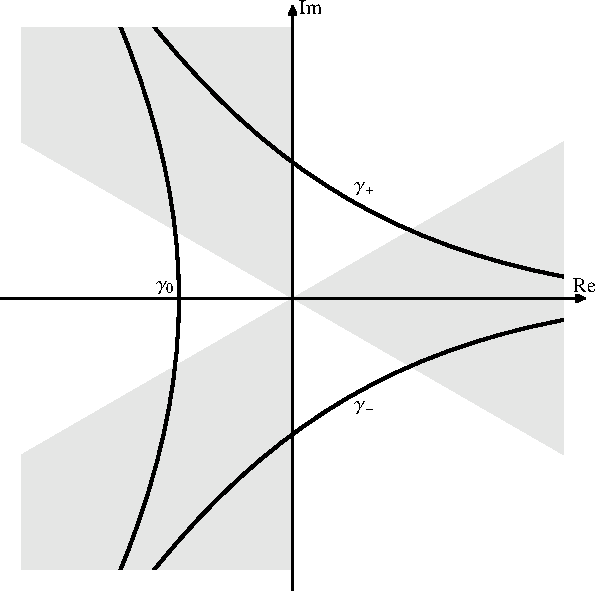
\includegraphics{chapters/images/airy-1.pdf}
\caption{Kurven zur Berechnung der Airy-Funktionen
\label{komplex:airy}}
\end{figure}
Als Beispiel soll die Airy-Differentialgleichung
\[
y''(x)-xy(x)=0
\]
gel"ost werden.
Wir nehmen an, dass die Differentialgleichung mit der Laplace-Transformation
gel"ost werden kann.
Allerdings verwenden wir nicht die Integration entlang der positiven
reellen Achse, wie das bei der traditionellen Laplace-Transformation
"ublich ist, sondern Integration eintlang eines beliebigen Weges in
der komplexen Ebene.
Wir nehmen also an, dass sich $y(x)$ schreiben l"asst als
\[
y(x)=\int_\gamma e^{xz}v(z)\,dz
\]
f"ur eine komplex differenzierbare Funktion $v(z)$ und eine Kurve
$\gamma\colon\mathbb R\to \mathbb C$.
Setzen wir diesen Ansatz in die Airy-Differentialgleichung ein,
erhalten wir
\begin{align*}
\int_\gamma z^2e^{xz}v(z)\,dz-\int\gamma xe^{xz}v(z)\,dz&=0
\end{align*}
Das zweite Integral kann mit partieller Integration umgeformt werden,
man erh"alt
\begin{align*}
\int\gamma xe^{xz}v(z)\,dz
&=
\int_{-\infty}^{\infty} xe^{x\gamma(t)}v(\gamma(t))\dot\gamma(t)\,dt
=
\left[e^{xz}v(z)\right]_{\gamma(-\infty)}^{\gamma(\infty)}
-\int_\gamma e^{xz}v'(z)\,dz
\end{align*}
Dieser Ausdruck ist nur dann sinnvoll, wenn der Weg $\gamma$ so gew"ahlt
wird, dass die Endpunkte des Weges der Integrand beliebig klein wird,
dies wird sp"ater die Wahl des Weges einschr"anken.
Andererseits erhalten wir die Differentialgleichung erster Ordnung
\begin{align*}
\int_\gamma e^{xz}(z^2v(z)+v'(z))\,dz=0
\qquad
\Rightarrow
\qquad
v'(z)+z^2v(z)=0
\end{align*}
f"ur $v(z)$, die mit Separation gel"ost werden kann:
\[
\int \frac{dv}{v}=-\int z^2\,dz
\qquad\Rightarrow\qquad
v(z)=-\frac13z^3.
\]
Setzen wir dies in den Ansatz f"ur $y(x)$ ein, finden wir
\[
y(x)=\int_\gamma e^{xz-\frac13z^3}\,dz.
\]
Jetzt muss die Kurve $\gamma$ so gew"ahlt werden, dass das Integral
wohldefiniert ist. 
Dazu muss der Realteil des Exponenten f"ur jedes beliebige reelle $x$ 
gegen $-\infty$ gehen, wenn $z$ gegen unendlich geht.
In Abbildung~\ref{komplex:airy} sind die Gebiete grau eingezeichnet,
in denen $-\frac13z^3$ negativen Realteil hat.
Zul"assige Wege m"ussen daher ``Enden'' in den grauen Gebieten haben,
d.~h.~$\gamma(t)$ muss in diesen Gebieten gegen Unendlich gehen, wenn
$t\to\pm\infty$.
Damit sind im Wesentlichen die drei Kurven $\gamma_0$, $\gamma_+$ und
$\gamma_-$ aus Abbildung~\ref{komplex:airy} w"ahlbar.

F"ur $x\to\infty$ w"achst $e^{xz}$ im positiven grauen Teilgebiet
"uber alle Grenzen, die Kurven $\gamma_+$ und $\gamma_-$ ergeben daher
eine unbeschr"ankte L"osung.
Nur die Kurve $\gamma_0$ kann ein beschr"ankte L"osung der Airy-Gleichung
geben.
Man nennt
\[
\operatorname{Ai}(x)
=
\frac{1}{2\pi i}\int_{\gamma_0} e^{xz-\frac13z^3}\,dz
\]
die Airy-Funktion.
Auf die Wahl der Kurve $\gamma_0$ kommt es nicht an, solange sie in den
beiden grauen Gebieten links der imagin"aren Achse enden.
Deformiert man die Kurve $\gamma_0$ in die imagin"are Achse, erh"alt
man daher die folgende Integraldarstellung der Airy-Funktion:
\begin{align*}
\operatorname{Ai}(x)
&=
\frac1{2\pi i}\int_{-\infty}^{\infty} e^{xit-\frac13(it)^3}i\,dt
\\
&=\frac{1}{2\pi i}\int_{-\infty}^{\infty} ie^{i(xt+\frac13t^3)}\,dt
\\
&=
\frac{1}{2\pi i}\int_{-\infty}^{\infty}
i\cos\biggl(xt+\frac13t^3\biggr)-\sin\biggl(xt+\frac13t^3\biggr)\,dt
\\
&=\frac{1}{\pi}\int_0^{\infty}\cos\biggl(xt+\frac13t^3\biggr)\,dt.
\end{align*}
Dabei haben wir im letzten Schritt verwendet, dass das Integral der
ungeraden Funktion $\sin(xt+\frac13t^3)$ "uber ein symmetrisches
Interval verschwindet.

Weitere Information "uber die Airy-Funktionen sind in \cite{skript:airy}
zusammengefasst.

\subsection{Die Cauchy-Integralformel}
Sei jetzt $f(z)$ eine komplex differenzierbare Funktion.
Dann ist auch die Funktion
\[
g(z)=\frac{f(z)}{z-a}
\]
komplex differenzierbar f"ur $z\ne a$.
Insbesondere ist der Wert des Wegintegrals von $g(z)$ entlang
eines geschlossenen Pfades um den Punkt $a$ unabh"angig von der Wahl
des Weges.
Zum Beispiel k"onnten wir das Wegintegral mit Hilfe eines kleinen Kreises
um $a$ mit Radius $r$ mit der Parametrisierung
\[
t\mapsto \gamma(t)=a+re^{it},\quad t\in[0,2\pi]
\]
berechnen.
Die Rechnung ergibt
\begin{align*}
\oint_\gamma \frac{f(z)}{z-a}\,dz
&=
\int_0^{2\pi} \frac{f(a+re^{it})}{re^{it}}ire^{it}\,dt
=
i\int_0^{2\pi} f(a+re^{it})\,dt
\end{align*}
Da $f(z)$ komplex differenzierbar ist, k"onnen wir $f(z)$ approximieren
durch $f(z)=f(a)+f'(a)(z-a)+o(z-a)$, also
\begin{align*}
\oint_{\gamma} \frac{f(z)}{z-a}\,dz
&=
i\int_0^{2\pi}f(a) + f'(a)re^{it}+o(r)\,dt
\\
&=
f(a)i\int_0^{2\pi}\,dt + irf'(a)\int e^{it}\,dt + i\int_0^{2\pi}o(r)\,dt
\\
&=
2\pi i f(a) + irf'(a)\underbrace{\left[\frac1{i}e^{it}\right]_0^{2\pi}}_{=0}+o(r)
\\
&=2\pi i f(a)+o(r).
\end{align*}
Da das Wegintegral einer komplex differenzierbaren Funktion aber unabh"angig
vom Weg und damit vom Radius $r$ sein muss, folgt
\[
\oint_\gamma \frac{f(z)}{z-a}\,dz=2\pi i f(a).
\]
Wir haben damit den folgenden Satz bewiesen:

\begin{satz}[Cauchy]
Ist $\gamma$ ein geschlossener Weg in der komplexen Ebene, die ein
Gebiet umrandet, in dem die komplexe Funktion $f(z)$ komplex
differenzierbar ist, dann gilt
\[
f(a)=\frac{1}{2\pi i}\oint_{\gamma}\frac{f(z)}{z-a}\,dz.
\]
Insbesondere sind die Werte einer komplex differenzierbaren Funktion 
im Inneren eines Gebietes durch die Werte auf dem Rand bereits vollst"andig
bestimmt.
\end{satz}

\subsubsection{Ableitungen und Cauchy-Formel}
Sei $f(z)$ eine komplex differenzierbare Funktion, als Definitionsgebiet
nehmen wir der Einfachheit halber einen Kreis vom Radius $r$ um den Nullpunkt,
sein Rand ist die Kurve $\gamma$.
Durch Ableiten der Cachyschen Integralformel finden wir
\begin{align*}
f(z)
&=
\frac1{2\pi i}\oint_{\gamma}\frac{f(\zeta)}{\zeta-z}\,d\zeta
\\
f'(z)
&=
\frac1{2\pi i}\oint_{\gamma}\frac{f(\zeta)}{(\zeta-z)^2}\,d\zeta
\\
f'' (z)
&=
\frac1{2\pi i}\oint_{\gamma}2\frac{f(\zeta)}{(\zeta-z)^3}\,d\zeta
\\
f'''(z)
&=
\frac1{2\pi i}\oint_{\gamma}2\cdot 3\frac{f(\zeta)}{(\zeta-z)^4}\,d\zeta
\\
&\vdots
\\
f^{(k)}(z)
&=
\frac{k!}{2\pi i}\oint_{\gamma}\frac{f(\zeta)}{(\zeta-z)^{k+1}}\,d\zeta
\end{align*}
Es folgt

\begin{satz}
Eine komplex differenzierbare Funktion ist beliebig oft differenzierbar.
\end{satz}

\subsubsection{Komplex differenzierbare Funktionen sind analytisch}
Wir haben fr"uher gesehen, dass Wegintegrale auf analytische Funktionen
f"uhren.
Andererseits zeigt das Cauchy-Integral, dass komplex differenzierbare
Funktionen durch genau die Integrale bestimmt sind, die in den
Reihenentwicklungen in Satz~\ref{komplex:integralanalytisch} auftraten.
Diese Resultate k"onnen wir im folgenden Satz zusammenfassen.

\begin{satz}
Eine komplex differenzierbare Funktion $f(z)$, die in einer Kreisscheibe
vom Radius $r$ um den Punkt $z_0$ definiert ist, ist analytisch.
Ihre Potenzreihenentwicklung
\[
f(z)=\sum_{k=0}^na_k(z-z_0)^k
\]
hat die Koeffizienten
\[
a_k=\frac1{2\pi i}\int_{\gamma}\frac{f(z)}{(z-z_0)^{k+1}}\,dz,\quad
k\ge 0
\]
\end{satz}

\begin{proof}[Beweis]
Da $f$ komplex differenzierbar ist, gilt
\[
f(z)=\frac1{2\pi i}\oint_\gamma \frac{f(\zeta)}{\zeta-z}\,d\zeta.
\]
In Satz~\ref{komplex:integralanalytisch} wurde gezeigt, dass $f(z)$
analytisch ist, und dass die Koeffizienten der Potenzreihe von
der verlangten Form sind.
\end{proof}

F"ur eine komplexe Funktion, die im Punkt $z_0$ eine Singularit"at hat,
also in einer Umgebung von $z_0$ ohne den Punkt $z_0$ definiert ist,
k"onnen wir das Resultat aus Satz~\ref{komplex:laurentreihe} verwenden,
und zum folgenden analogen Resultat gelangen:

\begin{satz}
Eine komplex differenzierbare Funktion $f(z)$, die in einer Kreisscheibe
vom Radius $r$ um den Punkt $z_0$ mit Ausnahme des Punktes $z_0$
definiert ist, kann in eine konvergente Laurent-Reihe
\[
f(z)=\sum_{k=-\infty}^{\infty} c_k(z-z_0)^k
\]
entwickelt werden, deren Koeffizienten durch
\[
c_k = \frac1{2\pi i}\oint\gamma \frac{f(\zeta)}{(z-z_0)^{k+1}}\,d\zeta,\qquad k\in\mathbb Z
\]
gegeben sind.
\end{satz}

%
% Analytische Fortsetzung
%
\section{Analytische Fortsetzung}
\subsection{Analytische Fortsetzung mit Potenzreihen}
\begin{figure}
\centering
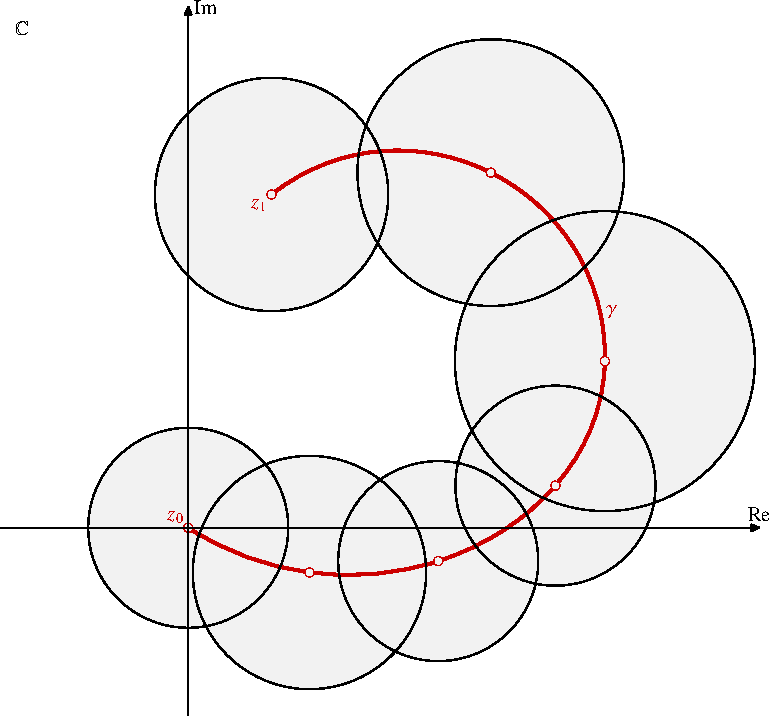
\includegraphics{chapters/images/komplex-1.pdf}
\caption{Analytische Fortsetzung einer komplexen Funktion entlang einer
Kurve $\gamma$.
\label{komplex:fortsetzung}}
\end{figure}
Eine komplex differenzierbare Funktion $f(z)$ ist immer darstellbar als
Potenzreihe, und ist daher analytisch.
So kann zum Beispiel die Funktion $1/z$ als Potenzreihe um jeden 
beliebigen Punkt $z_0$ entwickelt werden:
\begin{align}
f(z)
&=
\frac1z
=
\frac1{z_0-(z_0-z)}
=
\frac1{z_0}\cdot
\frac1{1-\displaystyle\frac{z_0-z}{z_0}}
=
\frac1{z_0}\sum_{k=0}^{\infty} \biggl(\frac{z_0-z}{z_0}\biggr)^k
=
\sum_{k=0}^{\infty} \frac{(-1)^k}{z_0^{k+1}} (z-z_0)^k,
\label{komplex:1durchreihe}
\end{align}
Die Koeffizienten dieser Potenzreihe sind
\[
a_k=\frac{(-1)^k}{z_0^{k+1}},
\]
und man kann den Konvergenzradius ausrechnen:
\[
\frac1{\varrho}
=
\limsup_{k\to\infty} \root{k}\of{|a_k|} = \lim_{k\to\infty}\frac1{|z_0|^{\frac{k+1}{k}}}
=
\frac1{|z_0|}.
\]
Der Konvergenzradius ist limitiert durch die Singularit"at bei an der Stelle
$z=0$.

Es gibt also keine einzelne Potenzreihe, die die Funktion $f(z)=\frac1z$ in der
ganzen komplexen Ebene darstellen kann.
W"ahlt man aber einzelne Punkte $z_0$ und $z_1$ derart, dass der Kreis
um $z_0$ mit Radius $|z_0|$ und der Kreis um $z_1$ mit Radius $|z_1|$
"uberlappen, dann werden die beiden Potenzreihen im "Uberlappungsgebiet
die gleichen Werte annehmen.

Man k"onnte allso eine Kurve $\gamma$ in der komplexen Ebene w"ahlen,
entlang der man in jedem Punkt die Funktion $f(z)$ in eine Potenzreihe 
entwickelt.
Liegen zwei Punkte nahe genug auf der Kurve $\gamma$, werden die
Konvergenzkreise der Potenzreihen "uberlappen, und die Potenzreihen
werden im "Uberlappungsgebiet die gleichen Werte liefern.

Selbst wenn man eine Funktion $f(z)$ nur in einem Kreis um den Punkt $z_0$
kennt, zum Beispiel durch eine Potenzreihe im Punkt $z_0$, kann man entlang
einer Kurve, die $z_0$ mit $z_1$ verbindet, in jedem Punkt eine Potenzreihe
finden, die mit der Potenzreihe in den Nachbarpunkten "ubereinstimmt, und
so die Definition der Funktion entlang dieser Kurve auf ein gr"osseres
Gebiet ausweiten, wie in Abbildung~\ref{komplex:fortsetzung} dargestellt.
Man nennt dies die {\em analytische Fortsetzung} der Funktion $f(z)$ 
entlange der Kurve $\gamma$.
\index{analytische Fortsetzung}
\index{Fortsetzung, analytische}

\begin{beispiel}
Wir haben bereits gesehen, dass sich die Funktion $f(z)=1/z$ in jedem
Punkt $z_0$ der komplexen Ebene in die Potenzreihe~\ref{komplex:1durchreihe}
entwickeln l"asst.
Diese Reihe l"asst sich integrieren
\[
F(z,z_0)
=
\sum_{k=0}^\infty\frac{(-1)^k}{(k+1)z_0^{k+1}}z^{k+1},
\]
diese Reihe ist ebenfalls auf einem Kreis vom Radius $|z_0|$ um den
Punkt $z_0$ konvergent.
Wir vermuten nat"urlich, dass dies eine Darstellung des nat"urlichen
Logarithmus einer komplexen Zahl ist.
Nat"urlich ist das immer nur auf einem Kreisgebiet m"oglich, die Reihe
f"ur $z_=1$ ist zum Beispiel im Punkt $z=-1$ nicht konvergent.

Um eine in der ganzen komplexen Ebene definierte Funktion $\log(z)$ zu
konstruieren, m"ussen wir also eine analytische Fortsetzung aufbauen.
Bei der Integration haben wir eine frei w"ahlbare Integrationskonstante
$C(z_0)$, die wir so w"ahlen m"ussen, dass die Reihen im "Uberlappungsgebiet
"ubereinstimmen:
\[
F(z,z_0) + C(z_0) = F(z,z_1)  + C(z_1)
\]
f"ur jedes $z$ im "Uberlappungsgebiet.
Dadurch wird aber nur die Differenz $C(z_1)-C(z_0)$ der Werte festgelegt.
Da wir "Ubereinstimmung mit der "ublichen Definition des Logarithmus
erreichen m"ochten, k"onnen wir $C(1)=0$ festlegen.

\begin{figure}
\centering
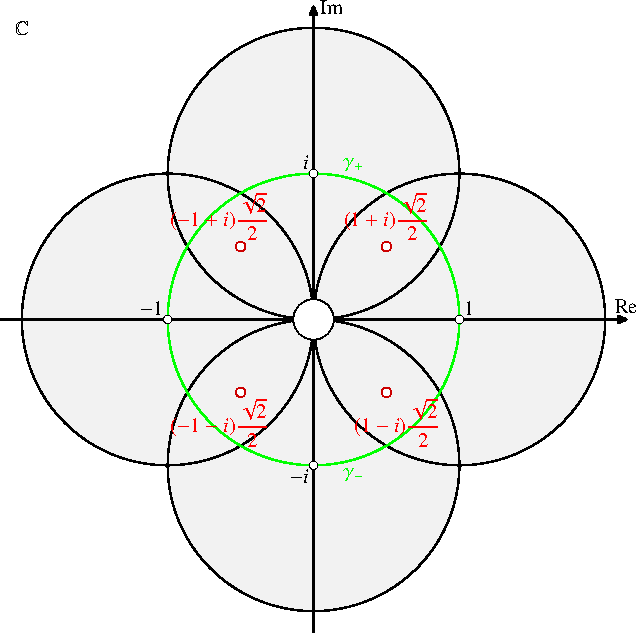
\includegraphics{chapters/images/komplex-2.pdf}
\caption{Analytische Fortsetzung f"ur die Funktion $\frac1z$ 
entlang der Pfade $\gamma_+$ und $\gamma_-$
\label{komplex:logfortsetzung}}
\end{figure}
Wir konstruieren jetzt die analytische Forstsetzung entlang der Kurven
$\gamma_+$ und $\gamma_-$ wie in Abbildung~\ref{komplex:logfortsetzung}
dargestellt.
Um die Differenz $C(z_1)-C(z_0)$ zu bestimmen, Werten wir die Funktionen
$F(z,z_0)$ und $F(z,z_1)$ jeweils im rot eingezeichneten Punkt aus.
Die exakte Berechnung ist etwas m"uhsam, da es sich ja nur um ein Beispiel
handelt, k"onnen wir die Reihen auch numerisch ausrechnen, und so die
Differenzen bestimmen:
\begin{align*}
&\text{Startpunkt $z_0=1$:}& C(1)&=0             &       &       \\
&\text{entlang $\gamma_+$:}& C(i)&= i\frac{\pi}2 & C(-1) &=  i\pi\\
&\text{entlang $\gamma_-$:}&C(-i)&=-i\frac{\pi}2 & C(-1) &= -i\pi
\end{align*}
Wir stellen fest, dass die analytische Fortsetzung der Logarthmusfunktion
entlang der Kurve $\gamma_+$ die Potenzreihe
\[
\log_+(z)
=
i\pi +\sum_{k=1}^\infty \frac{(-1)^{k+1}}{k(-1)^k}(z+1)^k
=
i\pi
-
\sum_{k=1}^\infty \frac{(z+1)^k}{k}
\]
ergibt, w"ahrend man entlang der  Kurve $\gamma_-$
\[
\log_-(z)
=
-i\pi +\sum_{k=1}^\infty \frac{(-1)^{k+1}}{k(-1)^k}(z+1)^k
=
-i\pi
-
\sum_{k=1}^\infty \frac{(z+1)^k}{k}
\]
findet.
Die beiden analytischen Fortsetzungen entlang der Kurven $\gamma_+$ und
$\gamma_-$ stimmen auf der negativen reellen Achse nicht "uberein,
sie unterscheiden sich um $2\pi i$:
\[
\log_+(z)-\log_-(z)=2\pi i.
\]
\end{beispiel}

Das Beispiel zeigt, dass es im Allgmeinen eine auf der ganzen komplexen
Ebene definierte komplexe Entsprechung einer reellen Funktion nicht
zu geben braucht.
Dieses Ph"anomen tritt zum Beispiel auch bei der Wurzelfunktion $f(z)=\sqrt{z}$
auf.
Diese Funktion ist im Punkt $z=0$ nicht differenzierbar, man muss diesen
Punkt also aus dem Definitionsbereich ausschliessen.
F"uhrt man man analog zum Beispiel eine analytische Fortsetzung durch,
findet man, dass sich die Werte von $f(z)$ f"ur die beiden Wege $\gamma_+$
und $\gamma_-$ durch das Vorzeichen unterscheiden.

\subsection{Analytische Fortsetzung mit Differentialgleichungen}
In Abschnitt~\ref{subsection:wegintegrale} wurde gezeigt, wie Wegintegrale
Stammfunktionen komplexer Funktionen liefern k"onnen.
Im vorangegangenen Abschnitt wurde untersucht, wie komplex differenzierbare
Funktionen mit Hilfe von analytischer Fortsetzung entlang einer Kurve
ausgedehnt werden kann.

Sei $f(z)$ eine komplex differenzierbare Funktion.
In jedem beliebigen Punkt des Definitionsbereichs k"onnen wir $f(z)$
in eine Potenzreihe entwickeln, und nat"urlich auch termweise integrieren.
Es gibt also in jedem Punkt $z_0$ des Definitionsbereichs eine
Funktion $F_{z_0}(z)$, die $F'_{z_0}(z)=f(z)$ erf"ullt.
Durch analytische Fortsetzung entlang einer Kurve $\gamma$ k"onnen
wir eine komplex differenzierbare Funktion $f(z)$ finden, die in einer
Umgebung der Kurve $F'(z)=f(z)$ erf"ullt.

Sei andererseits $\gamma\colon[a,b]\to\mathbb C$ eine Kurve in $\mathbb C$.
Dann k"onnen wir die Werte der Stammfunktion im Punkt $\gamma(b)$ durch
\[
F(\gamma(b)) = F(\gamma(a))+\int_\gamma f(z)\,dz
\]
berechnen.

\begin{beispiel}
Wir bestimmen die Stammfunktion von $f(z)=1/z$.
Entlang der reellen Achse weiss man bereits, dass die Stammfunktion
der nat"urliche Logarithmus ist, also $F(x)=\log x$.
Um diese Stammfunktion auf $\mathbb C$ auszudehnen, verwenden wir einen
kreisf"ormigen Pfad von der reellen Achse bis zum Punkt $z$.
Liegt $z$ in der oberen Halbebene, w"ahlen wir einen Pfad in der
oberen Halbebene, und umgekehrt.
Wir k"onnen die Zahl $z$ in Polarkoordinaten darstellen als $z=re^{i\varphi}$.
Ein Pfad von der reellen Achse kann mit
\[
\gamma\colon [0,1]\to\mathbb C: t\mapsto re^{it\varphi}
\]
parametrisiert werden.
Der Zuwachs der Stammfunktion entlang dieses Pfades ist
\[
F(z)-F(r)
=
\int_\gamma\frac1z\,dz
=
\int_0^1 \frac1{e^{it\varphi}}i\varphi e^{it\varphi}\,dt
=
i\varphi \int_0^1\,dt
=
i\varphi.
\]
Der Wert der Stammfunktion am Anfang der Kurve ist $\log r$, somit
folgt, dass
\[
\log z = \log r + i\varphi.
\qedhere
\]
\end{beispiel}

\section{"Ubungsaufgaben}
\begin{uebungsaufgaben}
\item
\input uebungsaufgaben/701.tex
\item
\input uebungsaufgaben/702.tex
\item
\input uebungsaufgaben/703.tex
\item
\input uebungsaufgaben/704.tex
\item
\input uebungsaufgaben/705.tex
\item
\input uebungsaufgaben/706.tex
\end{uebungsaufgaben}

